% ============================================================
%  HCMUT-DEE Thesis Kit v2.0.4 — Chương 3
%  Copyright (c) 2026 Nguyen Trong Thang & TS. Nguyen Phuc Khai
%  License: MIT
% ============================================================

\chapter{Hình Ảnh, Bảng Biểu \& Công Thức Toán}
\label{ch:figures-tables}

\section{Chèn hình ảnh}
\label{sec:figures}

\subsection{Hình ảnh đơn}

\begin{lstlisting}[style=latexstyle, caption={Chèn hình ảnh cơ bản}]
\begin{figure}[H]
  \centering
  \includegraphics[width=0.6\textwidth]{figures/examples/sample.png}
  \caption{Mo ta hinh anh}
  \label{fig:sample}
\end{figure}
\end{lstlisting}

\textbf{Các tùy chọn kích thước thường dùng:}
\begin{itemize}
  \item \verb|width=0.8\textwidth| --- 80\% chiều rộng văn bản
  \item \verb|width=10cm| --- Chính xác 10cm
  \item \verb|scale=0.5| --- Thu nhỏ 50\%
  \item \verb|height=5cm| --- Chiều cao 5cm
\end{itemize}

\textbf{Vị trí hình:} \verb|[H]| = chính xác tại đây, \verb|[htbp]| = để \LaTeX{} tự chọn vị trí tối ưu.

Ví dụ chèn hình đơn thực tế:
\begin{figure}[H]
  \centering
  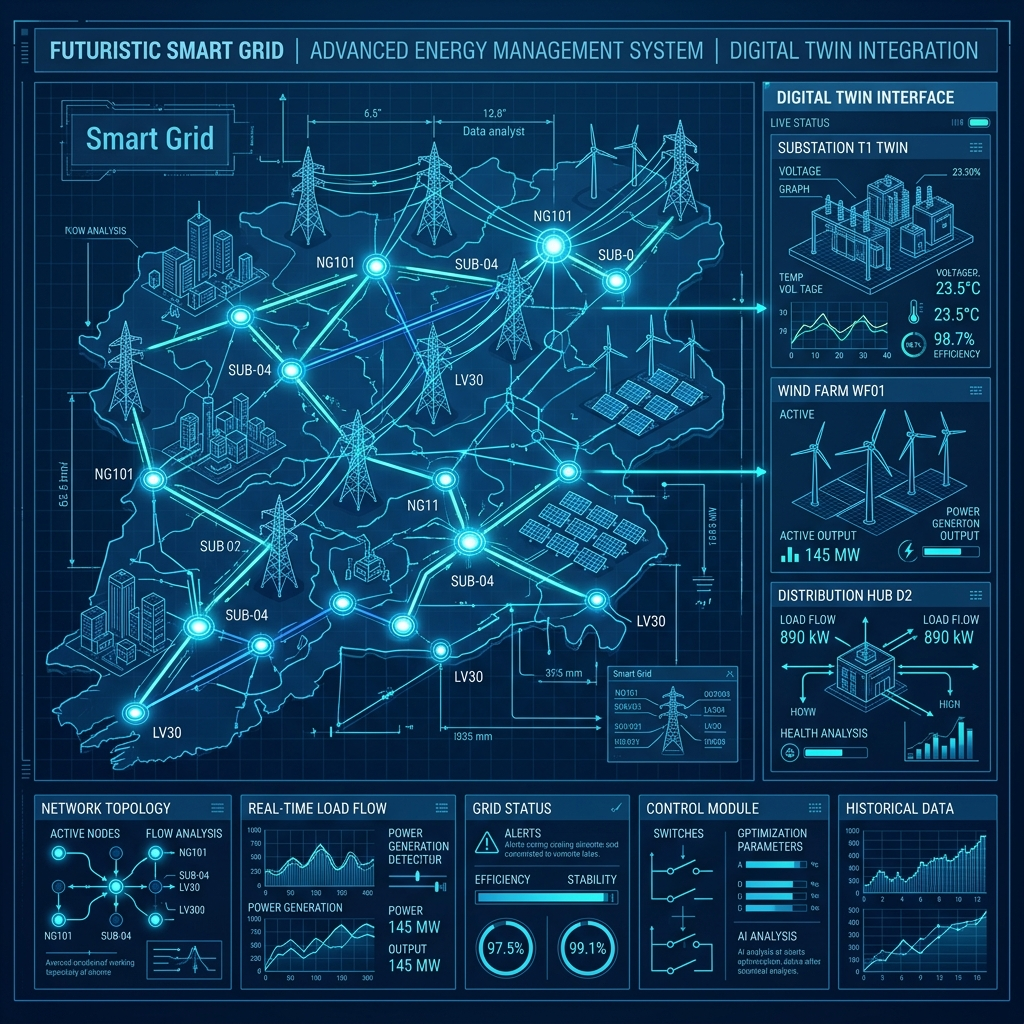
\includegraphics[width=0.6\textwidth]{figures/examples/smart_grid_ai.png}
  \caption{Mô hình trực quan hóa hệ thống lưới điện thông minh (Smart Grid)\protect\footnotemark}
  \label{fig:smart-grid-ai}
\end{figure}
\footnotetext{GHI CHÚ HỌC THUẬT QUAN TRỌNG: Hình ảnh minh họa này được tạo bởi AI (Generative AI). Theo quy định liêm chính học thuật, nếu sinh viên sử dụng hình ảnh do AI tạo sinh trong báo cáo/đồ án, BẮT BUỘC phải ghi rõ nguồn gốc trong chú thích hoặc footnote: \textit{"Hình ảnh được tạo bởi mô hình AI [Tên Model] với prompt chi tiết: [Nội dung prompt]"}. Ví dụ đối với hình này: Model: FLUX.1 / Prompt: \textit{"A futuristic high-tech Smart Grid power system with shining electrical nodes, transmission towers, and digital twins on a control dashboard interface, styled as a premium clean blueprint and technical schematic illustration..."}}

\subsection{Hình ảnh con (subfigure)}

\begin{lstlisting}[style=latexstyle, caption={Sử dụng subfigure}]
\begin{figure}[H]
  \centering
  \begin{subfigure}[b]{0.45\textwidth}
    \includegraphics[width=\textwidth]{hinh_a.png}
    \caption{Mo ta hinh a}
    \label{fig:sub-a}
  \end{subfigure}
  \hfill
  \begin{subfigure}[b]{0.45\textwidth}
    \includegraphics[width=\textwidth]{hinh_b.png}
    \caption{Mo ta hinh b}
    \label{fig:sub-b}
  \end{subfigure}
  \caption{Mo ta chung cho ca 2 hinh}
  \label{fig:both}
\end{figure}
\end{lstlisting}

Ví dụ chèn hệ hình con thực tế:
\begin{figure}[H]
  \centering
  \begin{subfigure}[b]{0.48\textwidth}
    \centering
    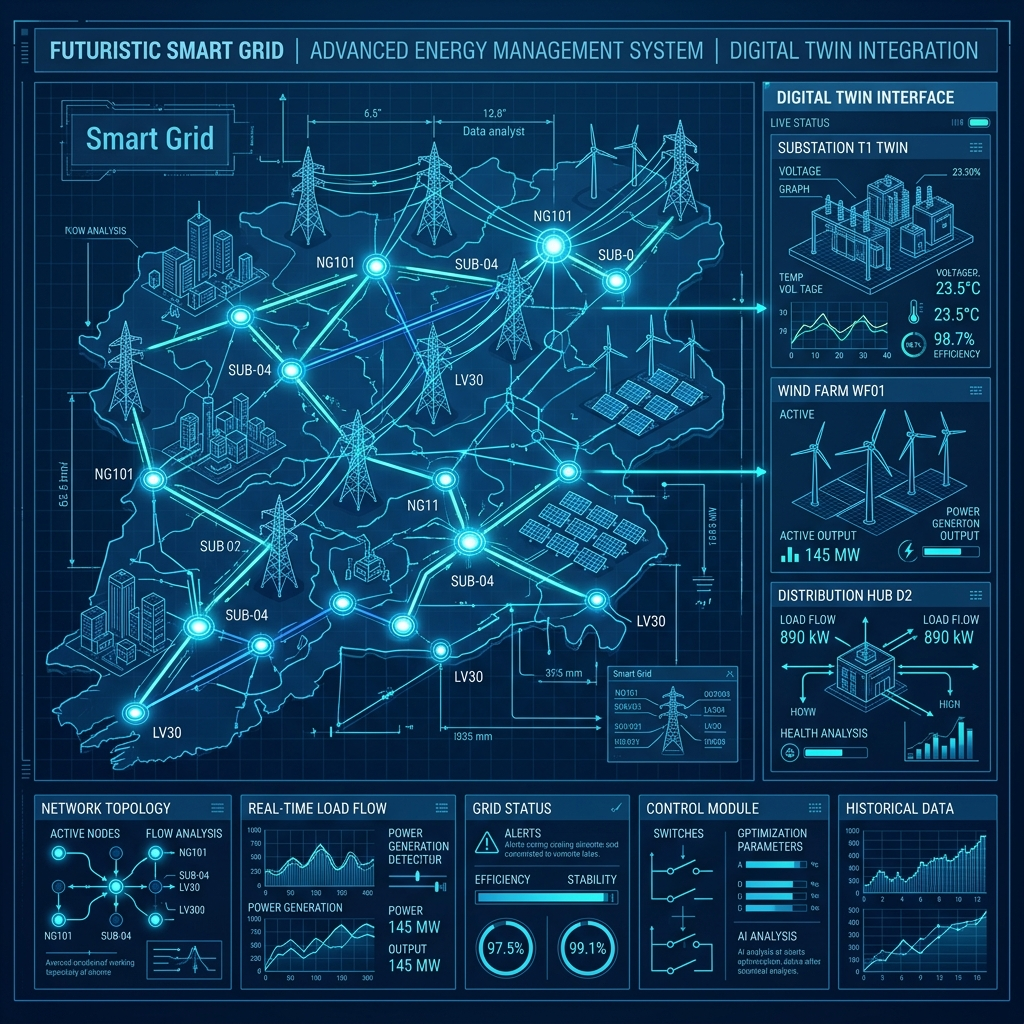
\includegraphics[width=\textwidth]{figures/examples/smart_grid_ai.png}
    \caption{Lưới điện thông minh}
    \label{fig:sub-smart-grid}
  \end{subfigure}
  \hfill
  \begin{subfigure}[b]{0.48\textwidth}
    \centering
    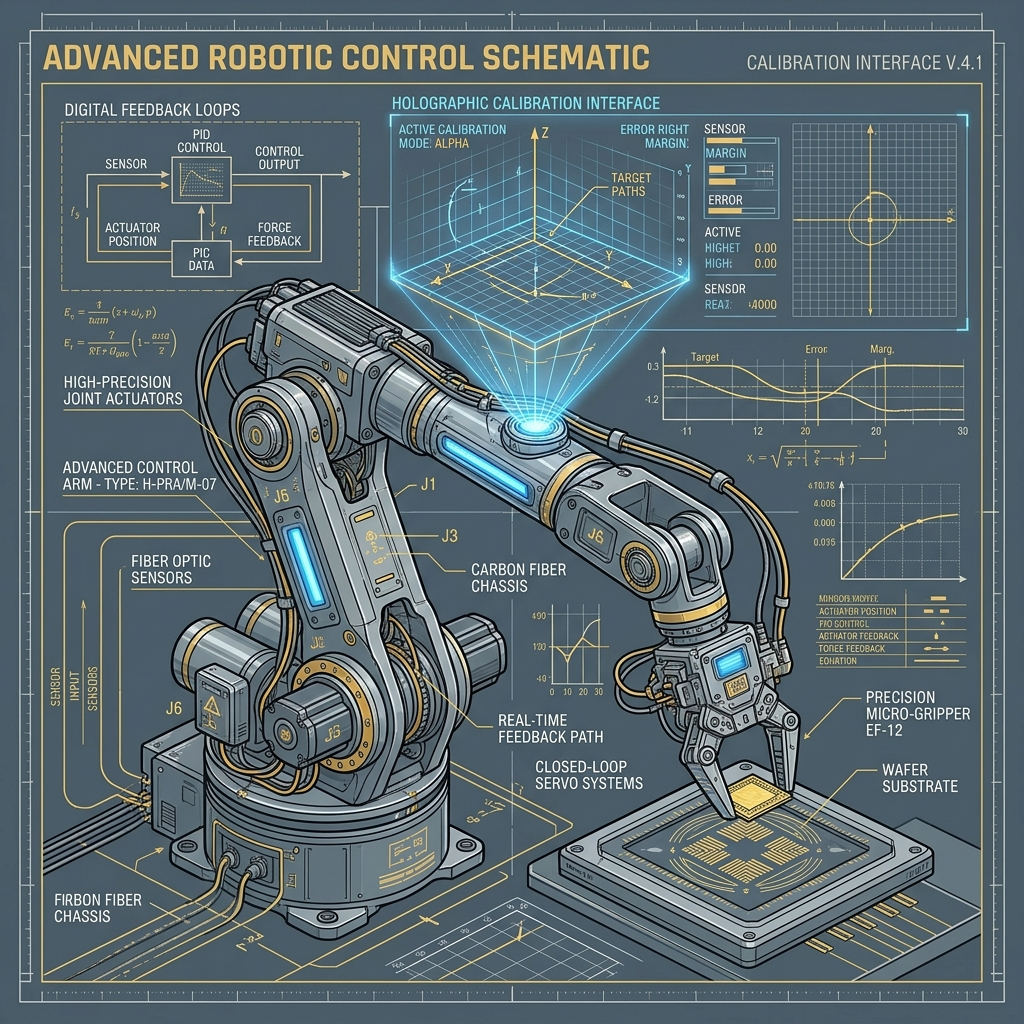
\includegraphics[width=\textwidth]{figures/examples/robotic_arm_ai.png}
    \caption{Cánh tay robot chính xác cao}
    \label{fig:sub-robotic-arm}
  \end{subfigure}
  \caption{Minh họa các thành phần hệ thống tự động hóa điện năng\protect\footnotemark}
  \label{fig:automation-components}
\end{figure}
\footnotetext{LƯU Ý LIÊM CHÍNH HỌC THUẬT VỀ HÌNH ẢNH AI: Tương tự như hình đơn, đối với hệ hình con (subfigure) có chứa ảnh do AI tạo sinh, sinh viên phải mô tả chi tiết nguồn gốc từng hình: (a) Lưới điện thông minh (Model: FLUX.1 / Prompt: \textit{"A futuristic high-tech Smart Grid..."}); (b) Cánh tay robot điều khiển (Model: FLUX.1 / Prompt: \textit{"A high-precision advanced robotic control arm..."}). Việc minh bạch nguồn gốc tài liệu là yếu tố sống còn trong nghiên cứu khoa học kỹ thuật.}

\subsection{Định dạng hình ảnh được hỗ trợ}

\begin{table}[H]
\centering
\caption{Các định dạng hình ảnh}
\label{tab:image-formats}
\begin{tabular}{llp{7cm}}
\toprule
\textbf{Định dạng} & \textbf{Khuyến nghị} & \textbf{Ghi chú} \\
\midrule
\texttt{.pdf} & $\bigstar\bigstar\bigstar$ & Vector, chất lượng cao nhất \\
\texttt{.eps} & $\bigstar\bigstar\bigstar$ & Vector, tự động chuyển sang PDF \\
\texttt{.png} & $\bigstar\bigstar$ & Bitmap, tốt cho ảnh chụp màn hình \\
\texttt{.jpg} & $\bigstar$ & Bitmap, tốt cho ảnh chụp, nén mất dữ liệu \\
\bottomrule
\end{tabular}
\end{table}

% ═══════════════════════════════════════════════════════════════
\section{Bảng biểu}
\label{sec:tables}

\subsection{Bảng đơn giản với booktabs}

\begin{lstlisting}[style=latexstyle, caption={Bảng với booktabs (khuyến nghị)}]
\begin{table}[H]
  \centering
  \caption{Ket qua thi nghiem}
  \label{tab:results}
  \begin{tabular}{lrr}
    \toprule
    \textbf{Phuong phap} & \textbf{Do chinh xac} & \textbf{Thoi gian} \\
    \midrule
    Phuong phap A & 95.2\% & 12.3s \\
    Phuong phap B & 97.8\% & 45.6s \\
    Phuong phap C & 96.5\% & 23.1s \\
    \bottomrule
  \end{tabular}
\end{table}
\end{lstlisting}

Ví dụ kết quả:

\begin{table}[H]
  \centering
  \caption{Kết quả thí nghiệm mẫu}
  \label{tab:sample-results}
  \begin{tabular}{lrr}
    \toprule
    \textbf{Phương pháp} & \textbf{Độ chính xác} & \textbf{Thời gian (s)} \\
    \midrule
    Phương pháp A & 95.2\% & 12.3 \\
    Phương pháp B & 97.8\% & 45.6 \\
    Phương pháp C & 96.5\% & 23.1 \\
    \bottomrule
  \end{tabular}
\end{table}

\subsection{Bảng dài (longtable)}

Dùng \texttt{longtable} cho bảng trải nhiều trang:

\begin{lstlisting}[style=latexstyle, caption={Bảng dài qua nhiều trang}]
\begin{longtable}{lll}
  \caption{Bang dai qua nhieu trang} \label{tab:long} \\
  \toprule
  \textbf{STT} & \textbf{Ten} & \textbf{Gia tri} \\
  \midrule
  \endfirsthead
  % Header lap lai o trang tiep theo
  \multicolumn{3}{c}{\textit{(Tiep theo trang truoc)}} \\
  \toprule
  \textbf{STT} & \textbf{Ten} & \textbf{Gia tri} \\
  \midrule
  \endhead
  1 & Muc 1 & 100 \\
  2 & Muc 2 & 200 \\
  % ... them cac dong khac
  \bottomrule
\end{longtable}
\end{lstlisting}

\subsection{Bảng ngang trang (landscape)}

\begin{lstlisting}[style=latexstyle, caption={Xoay bảng ngang trang}]
\begin{landscape}
\begin{table}
  \centering
  \caption{Bang rong can xoay ngang}
  \begin{tabular}{lllllllll}
    % ... noi dung bang rong ...
  \end{tabular}
\end{table}
\end{landscape}
\end{lstlisting}

% ═══════════════════════════════════════════════════════════════
\section{Công thức toán}
\label{sec:math}

\subsection{Công thức inline và display}

\begin{itemize}
  \item \textbf{Inline:} Dùng \verb|$...$| --- Ví dụ: $E = mc^2$
  \item \textbf{Display:} Dùng \verb|\[...\]| hoặc environment \texttt{equation}
\end{itemize}

\subsection{Công thức đánh số}

\begin{lstlisting}[style=latexstyle]
\begin{equation}
  P_{loss} = \sum_{k=1}^{N_{branch}} I_k^2 \cdot R_k
  \label{eq:ploss}
\end{equation}
\end{lstlisting}

Kết quả:
\begin{equation}
  P_{loss} = \sum_{k=1}^{N_{branch}} I_k^2 \cdot R_k
  \label{eq:ploss}
\end{equation}

Tham chiếu: ``Công thức~\eqref{eq:ploss} tính tổn thất công suất\ldots''

\subsection{Hệ phương trình (align)}

\begin{lstlisting}[style=latexstyle]
\begin{align}
  P_i &= V_i \sum_{j=1}^{N} V_j (G_{ij}\cos\theta_{ij}
         + B_{ij}\sin\theta_{ij}) \label{eq:pi} \\
  Q_i &= V_i \sum_{j=1}^{N} V_j (G_{ij}\sin\theta_{ij}
         - B_{ij}\cos\theta_{ij}) \label{eq:qi}
\end{align}
\end{lstlisting}

Kết quả:
\begin{align}
  P_i &= V_i \sum_{j=1}^{N} V_j (G_{ij}\cos\theta_{ij} + B_{ij}\sin\theta_{ij}) \label{eq:pi} \\
  Q_i &= V_i \sum_{j=1}^{N} V_j (G_{ij}\sin\theta_{ij} - B_{ij}\cos\theta_{ij}) \label{eq:qi}
\end{align}

\subsection{Ma trận}

\begin{lstlisting}[style=latexstyle]
\begin{equation}
  \mathbf{Y}_{bus} = \begin{bmatrix}
    Y_{11} & Y_{12} & \cdots & Y_{1n} \\
    Y_{21} & Y_{22} & \cdots & Y_{2n} \\
    \vdots & \vdots & \ddots & \vdots \\
    Y_{n1} & Y_{n2} & \cdots & Y_{nn}
  \end{bmatrix}
\end{equation}
\end{lstlisting}

Kết quả:
\begin{equation}
  \mathbf{Y}_{bus} = \begin{bmatrix}
    Y_{11} & Y_{12} & \cdots & Y_{1n} \\
    Y_{21} & Y_{22} & \cdots & Y_{2n} \\
    \vdots & \vdots & \ddots & \vdots \\
    Y_{n1} & Y_{n2} & \cdots & Y_{nn}
  \end{bmatrix}
  \label{eq:ybus}
\end{equation}

% ═══════════════════════════════════════════════════════════════
\section{Thuật toán (algorithm2e)}
\label{sec:algorithm}

\begin{lstlisting}[style=latexstyle, caption={Viết thuật toán}]
\begin{algorithm}[H]
  \caption{Ten thuat toan}
  \label{alg:sample}
  \KwIn{Du lieu dau vao}
  \KwOut{Ket qua dau ra}
  Khoi tao\;
  \For{$i = 1$ \KwTo $N$}{
    Tinh toan gia tri $f(x_i)$\;
    \If{$f(x_i) < f_{best}$}{
      $f_{best} \leftarrow f(x_i)$\;
    }
  }
  \Return $f_{best}$\;
\end{algorithm}
\end{lstlisting}

Ví dụ kết quả:

\begin{algorithm}[H]
  \caption{Thuật toán tối ưu hóa mẫu}
  \label{alg:sample}
  \KwIn{Quần thể ban đầu $X$, số vòng lặp $T_{max}$}
  \KwOut{Nghiệm tối ưu $x^*$}
  Khởi tạo quần thể ngẫu nhiên $X = \{x_1, x_2, \ldots, x_N\}$\;
  \For{$t = 1$ \KwTo $T_{max}$}{
    Tính giá trị hàm mục tiêu $f(x_i)$ cho mọi $i$\;
    \If{$f(x_i) < f_{best}$}{
      $x^* \leftarrow x_i$\;
      $f_{best} \leftarrow f(x_i)$\;
    }
    Cập nhật vị trí các cá thể\;
  }
  \Return $x^*$\;
\end{algorithm}
